\documentclass[10pt]{beamer}\usepackage[]{graphicx}\usepackage[]{color}
%% maxwidth is the original width if it is less than linewidth
%% otherwise use linewidth (to make sure the graphics do not exceed the margin)
\makeatletter
\def\maxwidth{ %
  \ifdim\Gin@nat@width>\linewidth
    \linewidth
  \else
    \Gin@nat@width
  \fi
}
\makeatother

\definecolor{fgcolor}{rgb}{0.345, 0.345, 0.345}
\newcommand{\hlnum}[1]{\textcolor[rgb]{0.686,0.059,0.569}{#1}}%
\newcommand{\hlstr}[1]{\textcolor[rgb]{0.192,0.494,0.8}{#1}}%
\newcommand{\hlcom}[1]{\textcolor[rgb]{0.678,0.584,0.686}{\textit{#1}}}%
\newcommand{\hlopt}[1]{\textcolor[rgb]{0,0,0}{#1}}%
\newcommand{\hlstd}[1]{\textcolor[rgb]{0.345,0.345,0.345}{#1}}%
\newcommand{\hlkwa}[1]{\textcolor[rgb]{0.161,0.373,0.58}{\textbf{#1}}}%
\newcommand{\hlkwb}[1]{\textcolor[rgb]{0.69,0.353,0.396}{#1}}%
\newcommand{\hlkwc}[1]{\textcolor[rgb]{0.333,0.667,0.333}{#1}}%
\newcommand{\hlkwd}[1]{\textcolor[rgb]{0.737,0.353,0.396}{\textbf{#1}}}%
\let\hlipl\hlkwb

\usepackage{framed}
\makeatletter
\newenvironment{kframe}{%
 \def\at@end@of@kframe{}%
 \ifinner\ifhmode%
  \def\at@end@of@kframe{\end{minipage}}%
  \begin{minipage}{\columnwidth}%
 \fi\fi%
 \def\FrameCommand##1{\hskip\@totalleftmargin \hskip-\fboxsep
 \colorbox{shadecolor}{##1}\hskip-\fboxsep
     % There is no \\@totalrightmargin, so:
     \hskip-\linewidth \hskip-\@totalleftmargin \hskip\columnwidth}%
 \MakeFramed {\advance\hsize-\width
   \@totalleftmargin\z@ \linewidth\hsize
   \@setminipage}}%
 {\par\unskip\endMakeFramed%
 \at@end@of@kframe}
\makeatother

\definecolor{shadecolor}{rgb}{.97, .97, .97}
\definecolor{messagecolor}{rgb}{0, 0, 0}
\definecolor{warningcolor}{rgb}{1, 0, 1}
\definecolor{errorcolor}{rgb}{1, 0, 0}
\newenvironment{knitrout}{}{} % an empty environment to be redefined in TeX

\usepackage{alltt}
% \usetheme{jhsph}
\usepackage[T1]{fontenc}
\setcounter{secnumdepth}{3}
\setcounter{tocdepth}{3}
\usepackage{url}
\usepackage{graphicx}
\usepackage{multimedia}
\ifx\hypersetup\undefined
  \AtBeginDocument{%
    \hypersetup{unicode=true,pdfusetitle,
 bookmarks=true,bookmarksnumbered=false,bookmarksopen=false,
 breaklinks=false,pdfborder={0 0 0},pdfborderstyle={},backref=false,colorlinks=false}
  }
\else
  \hypersetup{unicode=true,pdfusetitle,
 bookmarks=true,bookmarksnumbered=false,bookmarksopen=false,
 breaklinks=false,pdfborder={0 0 0},pdfborderstyle={},backref=false,colorlinks=false}
\fi
\usepackage{breakurl}

\makeatletter

%%%%%%%%%%%%%%%%%%%%%%%%%%%%%% Textclass specific LaTeX commands.
 % this default might be overridden by plain title style
 \newcommand\makebeamertitle{\frame{\maketitle}}%
 % (ERT) argument for the TOC
 \AtBeginDocument{%
   \let\origtableofcontents=\tableofcontents
   \def\tableofcontents{\@ifnextchar[{\origtableofcontents}{\gobbletableofcontents}}
   \def\gobbletableofcontents#1{\origtableofcontents}
 }


\usetheme{PaloAlto}

\makeatother
\IfFileExists{upquote.sty}{\usepackage{upquote}}{}
\begin{document}

\title[]{Accelerometry: Data structure and analysis}
\author[]{Andrew Leroux \& Jacek K Urbanek \& Ciprian Crainiceanu}
\makebeamertitle




\section{Background}

\begin{frame}
\frametitle{Accelerometry: Objectively Measured Physical Activity}
\begin{itemize}
\item What are wearable and implantable devices?
\item Why do we care?
\item Overview of accelerometry data 
    \begin{itemize}
    \item Micro-scale (raw, sub-second) data
    \item Macro-scale data
    \end{itemize}
\item Working with publicly accelerometry data in NHANES
\end{itemize}
\end{frame}


\subsection{Wearable and Implantable Devices}


% \section{Weabale}
\begin{frame}
\frametitle{Wearable and Implantable Technology}
\begin{itemize}
\item Wearable and implantable devices are smart electronic devices that can be worn on the body as implants or accessories
\item Emerging technology (increasing variety of sensors and signals measured)
\item Growing popularity in health research and consumer tech
\end{itemize}
\end{frame}


\begin{frame}
\frametitle{Why Do We Care?}
\begin{itemize}
\item Prediction of mortality: simple summary features predict 5-year mortality better than age (walk through this analysis later)
\item Self-reported PA shown to be associated with many positive health outcomes
    \begin{itemize}
    \item Recall bias
    \item Low/moderate correlation with objectively measured PA
    \end{itemize}
\end{itemize}
\end{frame}


\begin{frame}
\frametitle{Accelerometry}
\begin{itemize}
\item Accelerometry: non-invansive monitoring of (a proxy of) activity using accelerometers
\item Accelerometer: device which measures acceleration
\end{itemize}
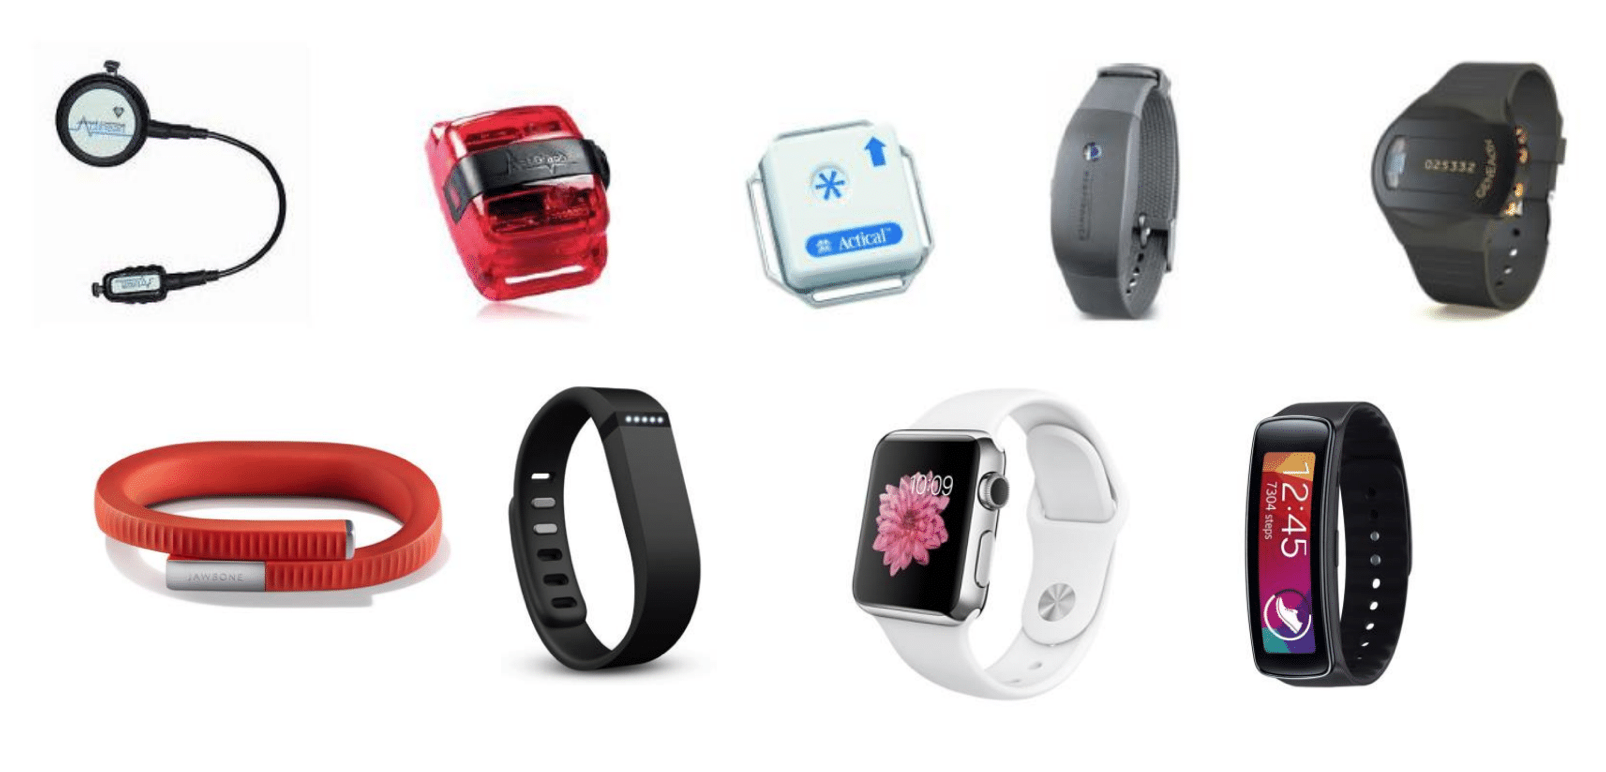
\includegraphics[width=\textwidth]{accelerometers_example}
\end{frame}







\begin{frame}
\frametitle{Other Wearables/Implabtables}
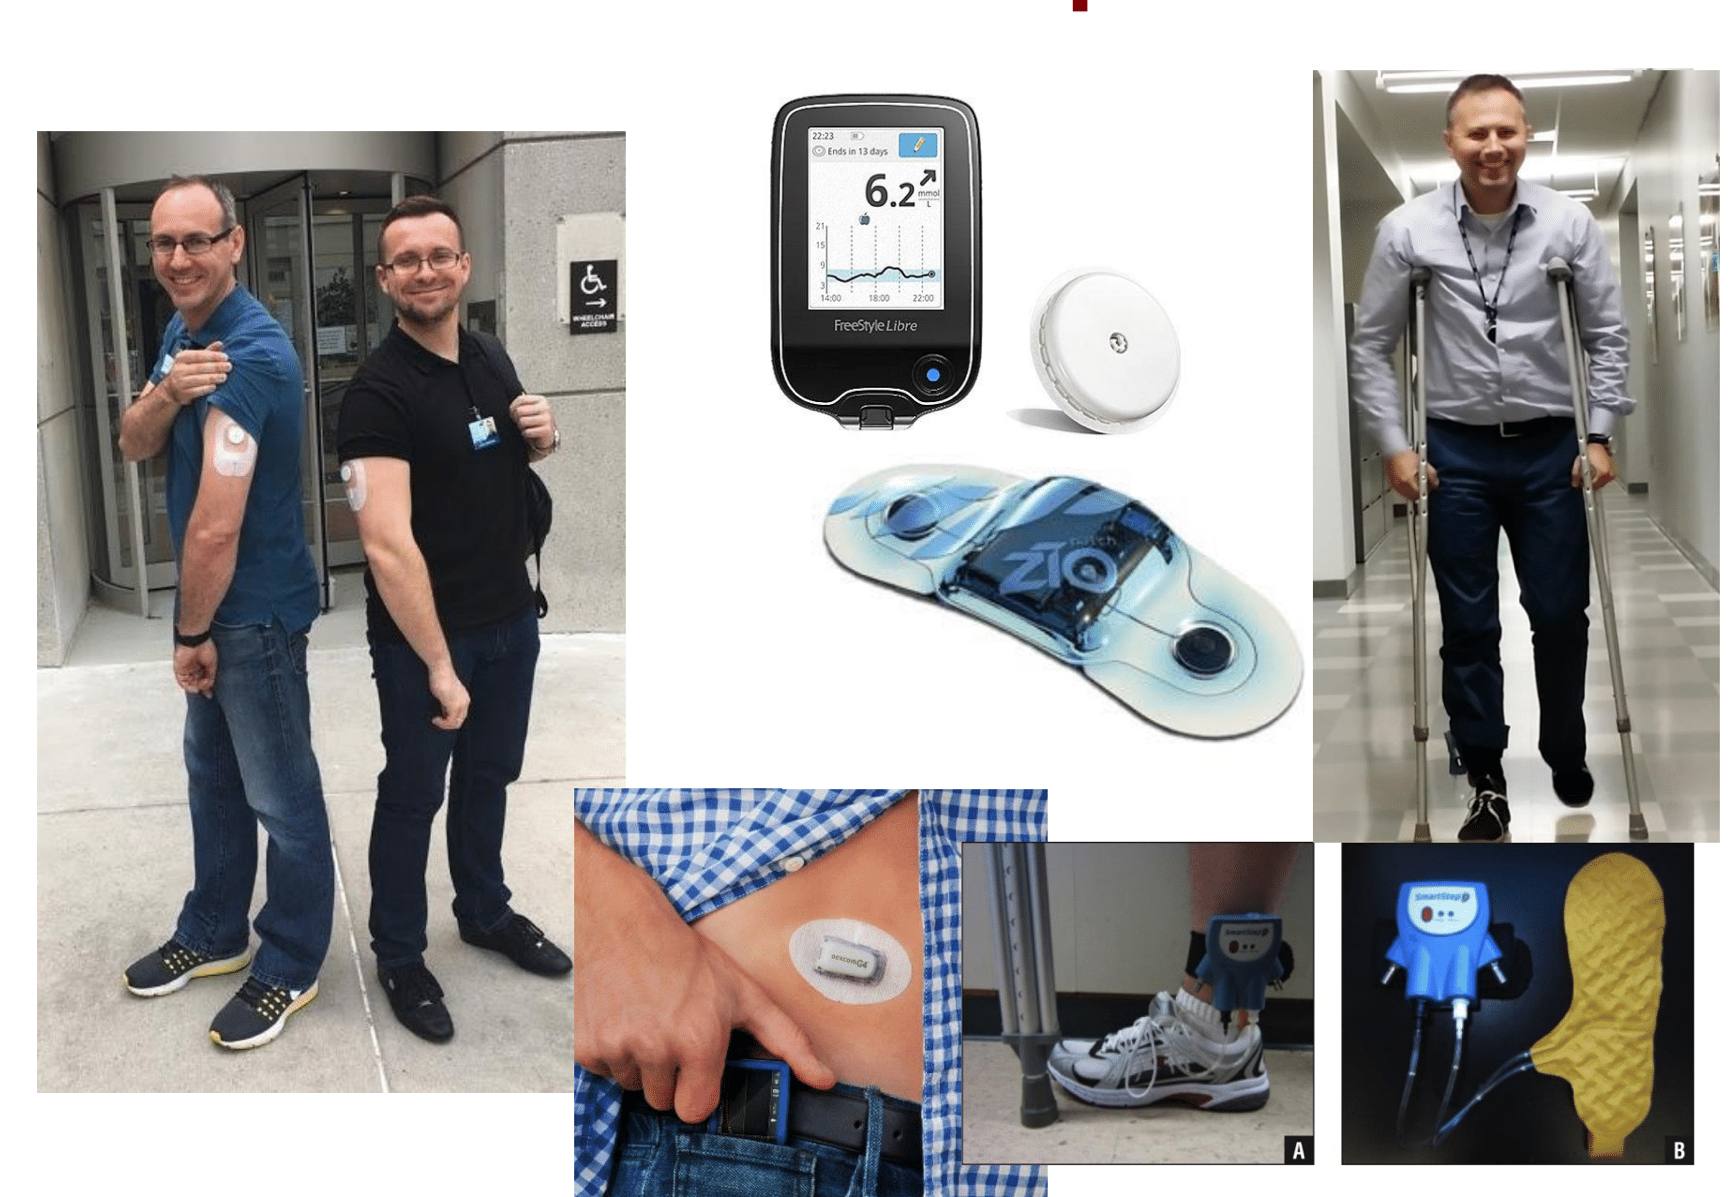
\includegraphics[width=\textwidth]{wearables_example}
\end{frame}


\begin{frame}
\frametitle{Scientific Questions}
\begin{itemize}
\item Physical activity and health (mortality, comorbidities, etc.)\footnotemark
\item Epidemiology of aging\footnotemark
\item Circadian rhythms\footnotemark
\item Sleep quality\footnotemark
\end{itemize}

\footnotetext{Leroux A, Di J, Smirnova E, et al. Organizing and Analyzing the Activity Data in NHANES. Statistics in Biosciences. 2019. 10.1007/s12561-018-09229-9.}
\footnotetext{Varma VR, Dey D, Leroux A, et al. Re-evaluating the effect of age on physical activity over the lifespan. Prev Med. 2017;101:102-108.}
\footnotetext{Xiao L, Huang L, Schrack JA, et al. Quantifying the lifetime circadian rhythm of physical activity: a covariate-dependent functional approach. Biostatistics. 2014;16(2):352-67.}
\footnotetext{Jacek K. Urbanek, Adam P. Spira, et al. Epidemiology of objectively measured bedtime and chronotype in US adolescents and adults: NHANES 2003–2006. Chronobiology International. 2018;35(3):416-434}
\end{frame}





\subsection{Overview of Accelerometry Data}

\begin{frame}
\frametitle{Measurement}

\begin{itemize}
\item Accelerometers are used to quantify "PA" as 
    \begin{itemize}
    \item Activity counts 
    \item Number of steps 
    \item Number of calories burned
    \end{itemize}
\end{itemize}
\end{frame}



\begin{frame}
\frametitle{Accelerometry in Action}
% \movie[width=8cm,height=4.5cm]{Ciprian wrist accelerometers}{AccVideo_Crainiceanu_Urbanek_720.mov}
\movie[width=10cm,height=7cm]{Wrist + Ankle accelerometer video}{AccVideo_Karas_Urbanek.avi}
\end{frame}



\begin{frame}
\frametitle{Major Data Challenges}
\begin{itemize}
\item Size
\item Complexity and heterogeneity
\item Lack of standardized data collection protocols
    \begin{itemize}
    \item Device type
    \item Device location 
    \item Wear/non-wear compliance
    \item Number of days of observation
    \end{itemize}
\end{itemize}
\end{frame}


\begin{frame}
\frametitle{Raw Accelerometry Data}
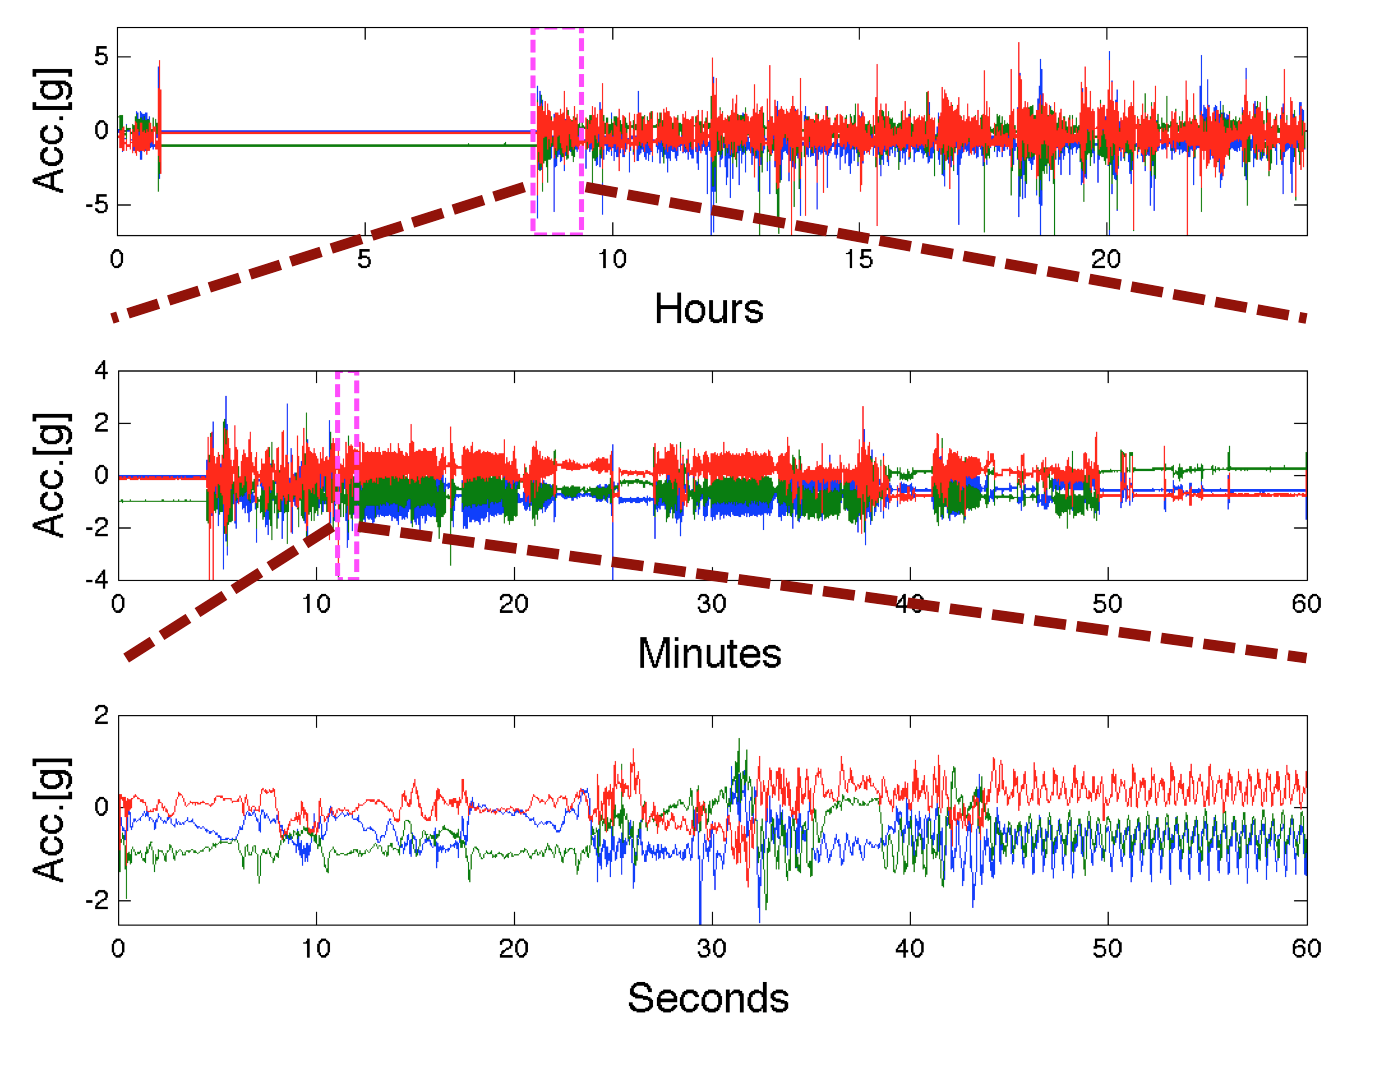
\includegraphics[width=\textwidth]{raw_accel_data_pt1}
\end{frame}

\begin{frame}
\frametitle{Raw Accelerometry Data}
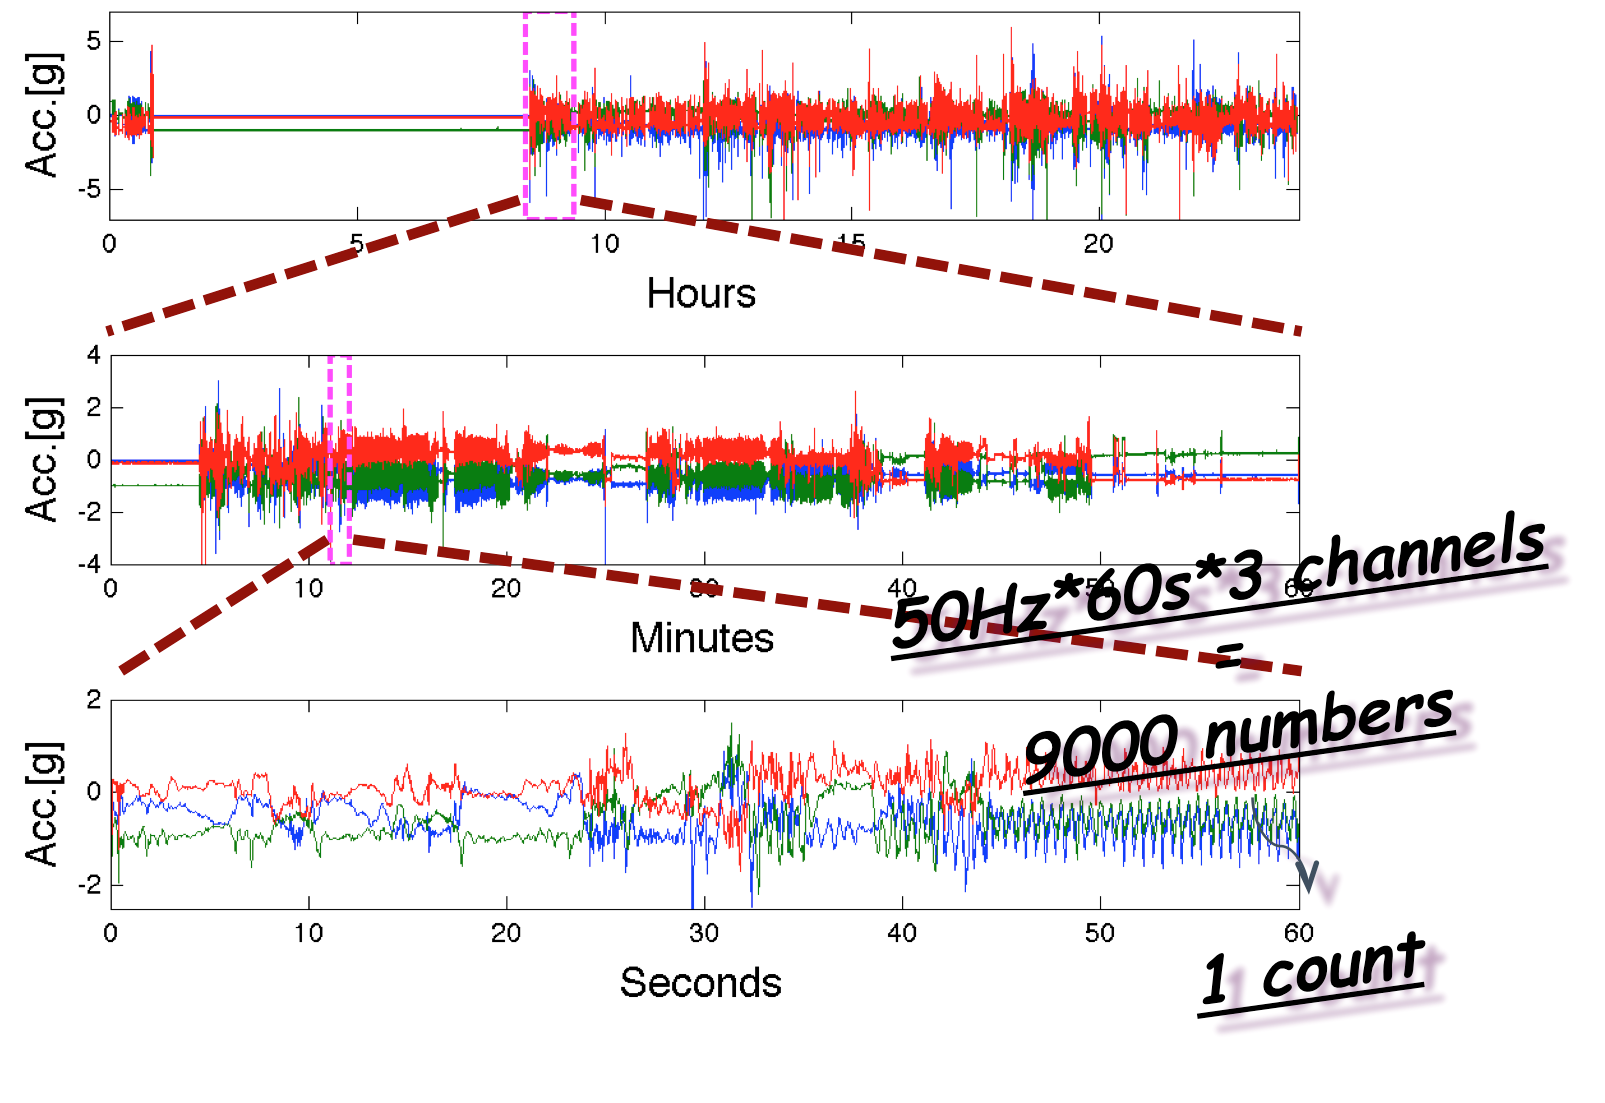
\includegraphics[width=\textwidth]{raw_accel_data_pt2}
\end{frame}













\begin{frame}
\frametitle{Micro- vs Macro-Scale Accelerometry Data}
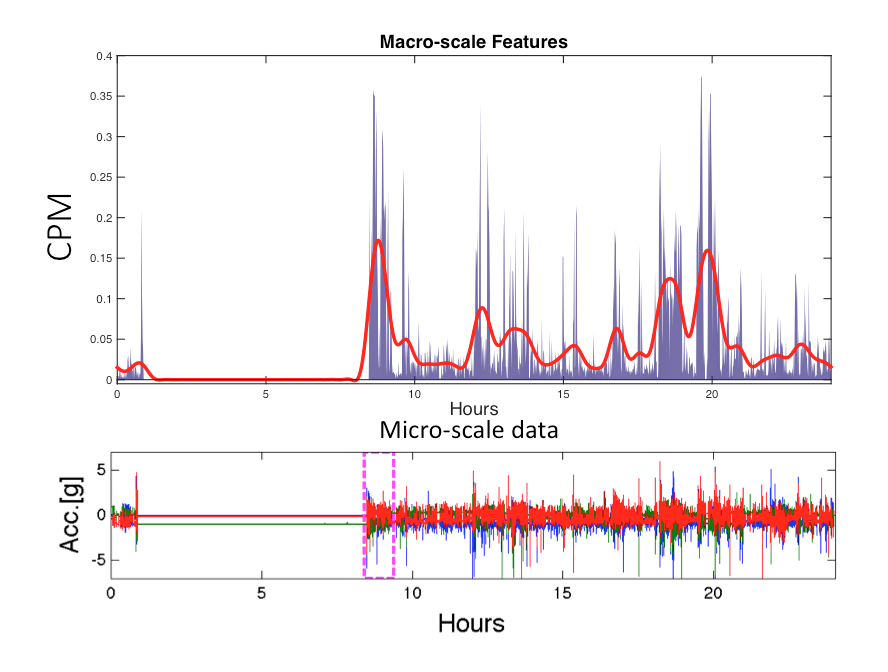
\includegraphics[width=\textwidth]{micro_vs_macro_accel_data}
\end{frame}


\begin{frame}
\frametitle{Macro Scale Accelerometry Data: Compliant Participant}
\centering
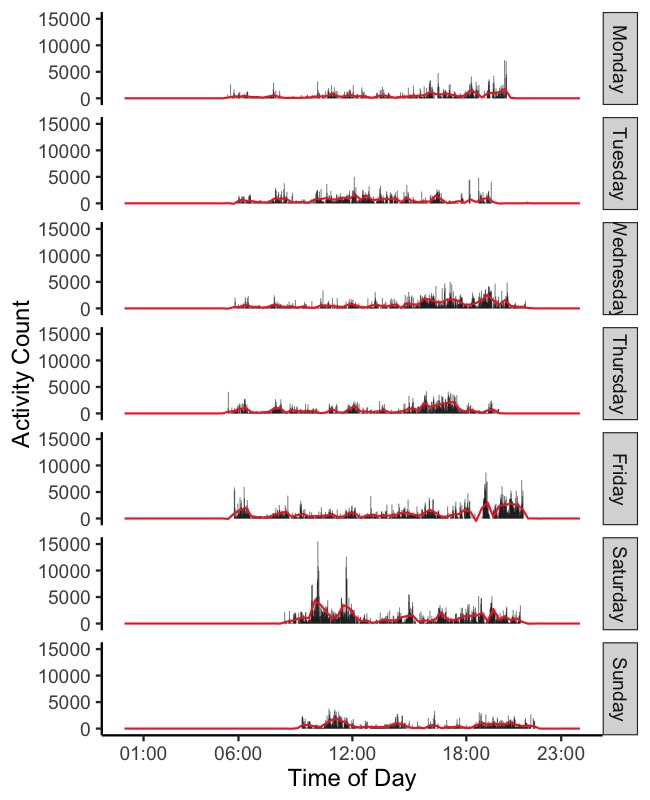
\includegraphics[height=\textheight]{profile_id1}
\end{frame}

\begin{frame}
\frametitle{Macro Scale Accelerometry Data: Non-Compliant Participant}
\centering
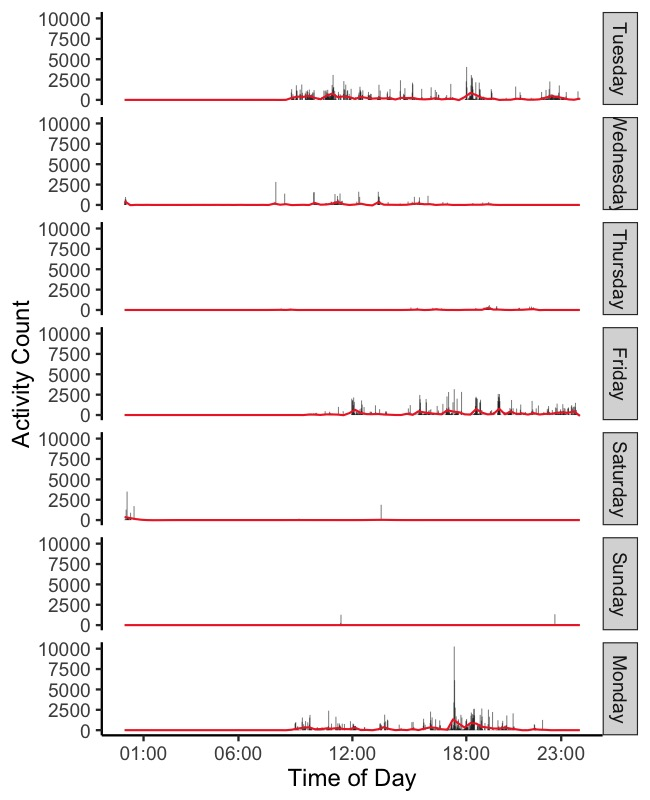
\includegraphics[height=\textheight]{profile_id2}
\end{frame}


\begin{frame}
\frametitle{Macro Scale Accelerometry Data}
\begin{itemize}
\item Easier to see patterns visually
\item Still "big" data! 1440 obs/day $\times$ 7 days. Can we reduce the dimension of the data further?
\item Common appraoch: calculate a single (scalar) summary measure per day of "good" data, 
average across days within a subject (more on this later)

\end{itemize}
\end{frame}












\section{Application: NHANES}

\begin{frame}
\frametitle{NHANES accelerometry: Reproducing these Analyses}
\begin{itemize}
\item All analyses presented here can be replicated using the "CSS\_NHANES.R" script located at 
\url{https://www.github.com/andrew-leroux/CSS_NHANES/}
\item Steps:
    \begin{itemize}
    \item Download or clone
    \item Open R project ("CSS\_NHANES.Rproj")
    \item Open R script "CSS\_NHANES.R"
    \item Run code
    \end{itemize}
\end{itemize}
\end{frame}




\begin{frame}
\frametitle{NHANES accelerometry}
\begin{itemize}
\item The National Health and Nutrition Survey is a cross-sectional study of the US population performed in 2-year waves
\item Complex survey structure (beyond the scope of this talk)
\item Accelerometry data available for the 2003-2004 and 2005-2006 waves
    \begin{itemize}
    \item Acceleration summarized into minute-level "activity counts"
    \item Up to 7 days of data for each participant
    \item Study protocol: remove the device at bedtime 
    \end{itemize}
\end{itemize}
\end{frame}



\begin{frame}
\frametitle{NHANES accelerometry: data structure}
\begin{itemize}
\item Accelerometry data downloadble from NHANES is in long format
\item Very large file sizes ($\approx$ 2.5 GB)
\item Unintuitive data structure
\end{itemize}
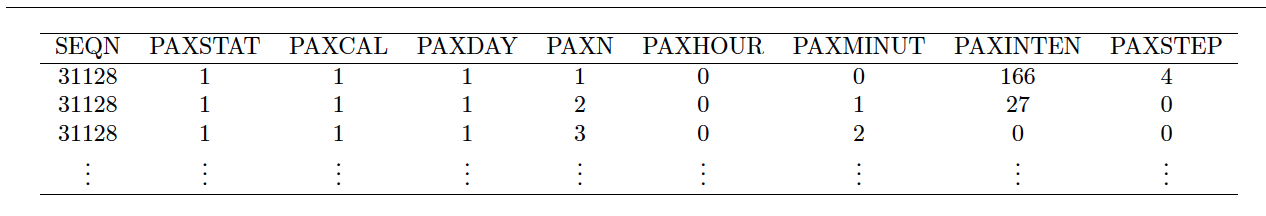
\includegraphics[width=\textwidth]{accel_data_long}
\end{frame}





\section{An NHANES data package}


\begin{frame}
\frametitle{NHANES accelerometry: proposed data strucutre}
\begin{itemize}
\item Wide format instead of long format\footnotemark ($\approx$ 60 MB)
\item 7 rows per participant, descending cronologoical order
\end{itemize}
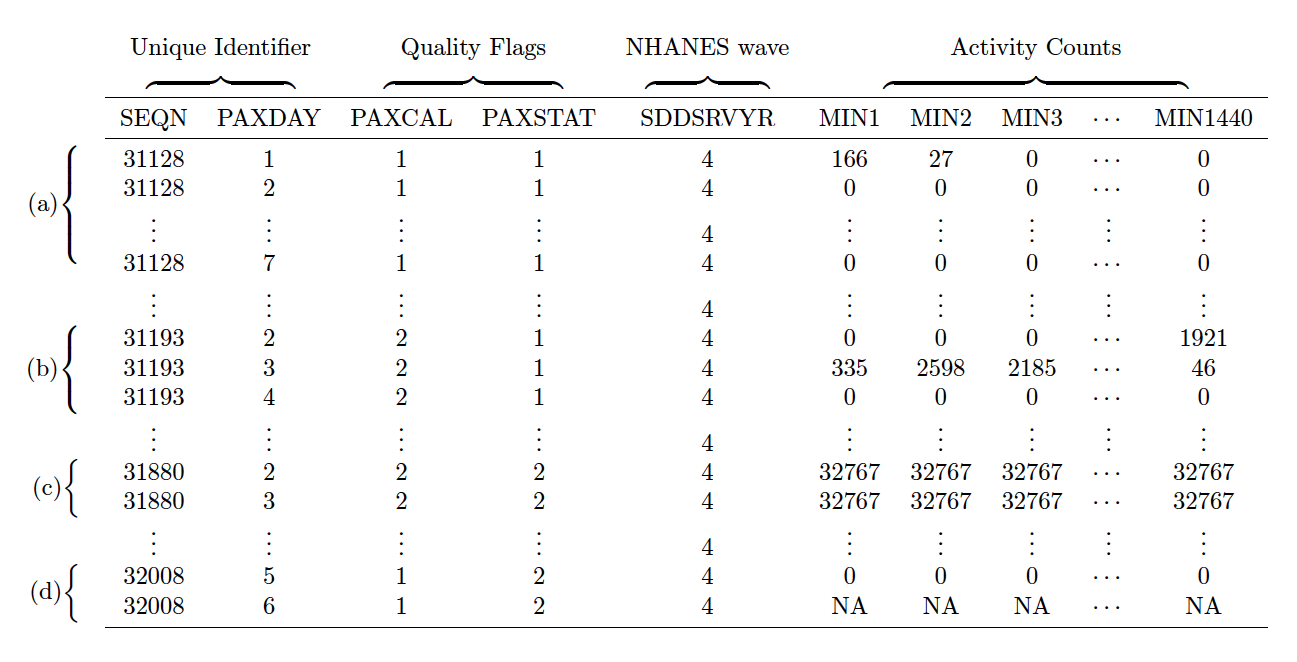
\includegraphics[width=\textwidth]{accel_data_wide}
\footnotetext{Leroux A, Di J, Smirnova E, et al. Organizing and Analyzing the Activity Data in NHANES. Statistics in Biosciences. 2019. 10.1007/s12561-018-09229-9.}
\end{frame}



\begin{frame}
\frametitle{NHANES accelerometry: {\it rnhanesdata} package}
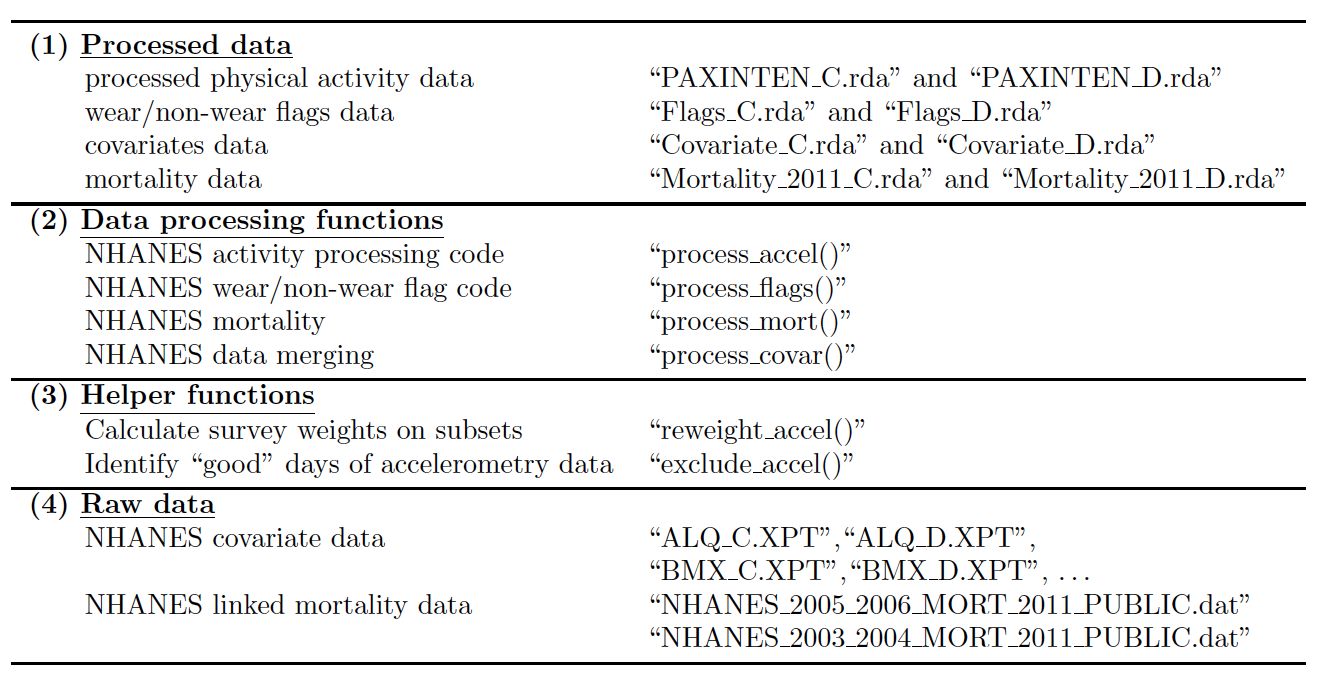
\includegraphics[width=\textwidth]{rnhanesdata}
\footnotetext{Leroux A, Di J, Smirnova E, et al. Organizing and Analyzing the Activity Data in NHANES. Statistics in Biosciences. 2019. 10.1007/s12561-018-09229-9.}
\end{frame}


\begin{frame}[fragile]
\frametitle{rnahnesdata: Package Installation}

\begin{itemize}
\item Package installation may take a few minutes due to the size of the processed data.
\item Requires the devtools package 
\item See ?"rnhanesdata-package" for details
\end{itemize}

\begin{knitrout}\small
\definecolor{shadecolor}{rgb}{0.969, 0.969, 0.969}\color{fgcolor}\begin{kframe}
\begin{alltt}
\hlkwa{if}\hlstd{(}\hlopt{!}\hlkwd{require}\hlstd{(}\hlstr{"rnhanesdata"}\hlstd{))\{}
    \hlstd{devtools}\hlopt{::}\hlkwd{install_github}\hlstd{(}\hlstr{"andrew-leroux/rnhanesdata"}\hlstd{)}
    \hlkwd{require}\hlstd{(}\hlstr{"rnhanesdata"}\hlstd{)}
\hlstd{\}}
\end{alltt}
\end{kframe}
\end{knitrout}
\end{frame}



\section{EDA}




\begin{frame}
\frametitle{NHANES accelerometry: Analysis Procedure}
\begin{itemize}
\item Load and merge any relevant data by unique identifier (SEQN)
\item Apply exclusion criteria
    \begin{itemize}
    \item Data quality: 1) device calibration (PAXCAL); and 2) NHANES supplied flag (PAXSTAT)
    \item Adherence to wear-time protocol. Most studies use $\geq 10$ hours.
    \item Sufficient number of days of data. Most studies use $ \geq 3$ days of data with $\geq 10$ hours of wear.
    \item Other criteria: missing data, etc.
    \end{itemize}   
\item Calculate features of interest
\item Incorporate survey design? Survey weights?
\item Regresison, machine learning, etc.
\end{itemize}
\end{frame}




\subsection{Compliance}

\begin{frame}
\frametitle{NHANES accelerometry: Compliance}
\begin{itemize}
\item Given our estimated wear/non-wear time algorithm, how much data do we lose?
\item Generally, scalar features are derived from individuals' activity. 
\item Idea: we are attempting to estimate "long-term average" levels (or patterns) of activity
\item Differential day-of-week compliance?
    \begin{itemize}
    \item People tend to be less active on the weekends 
    \item If certain groups of people disproportionately refuse/forget to wear the device on weekends,
            overestimate that group's average activity
    \end{itemize}
\end{itemize}
\end{frame}




\begin{frame}
\frametitle{NHANES accelerometry: Compliance}
\begin{itemize}
\item Age is one of the most important confounders in most epidemiologic analyses
\item Visualize distribution of age by day of week for "good" data
\end{itemize}
\begin{center}
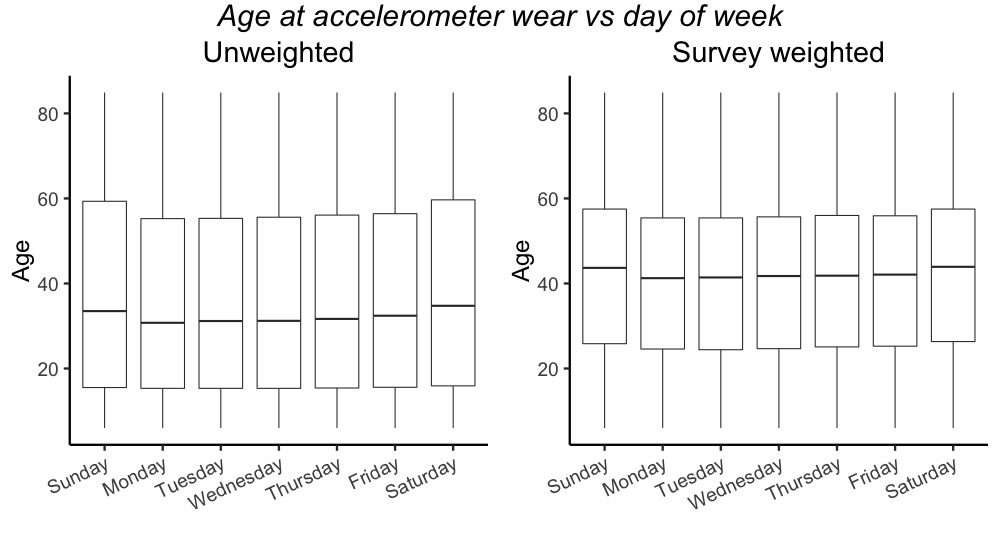
\includegraphics[width=\textwidth]{wear_time_by_dow}
\end{center}
\end{frame}



\begin{frame}
\frametitle{NHANES accelerometry: Compliance}
\begin{itemize}
\item Plot number of days of "good" accelerometry data versus age
\item Some evidence of differential day-of-week compliance by age. This is generally ignored in practice! 
\end{itemize}
\begin{center}
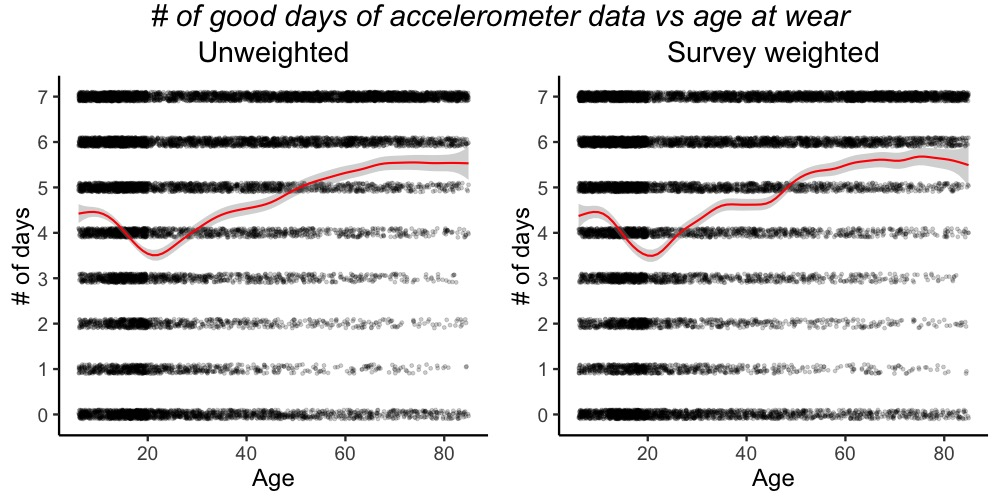
\includegraphics[width=\textwidth]{ndays_accel_by_age}
\end{center}
\end{frame}


\begin{frame}
\frametitle{NHANES accelerometry: Compliance}
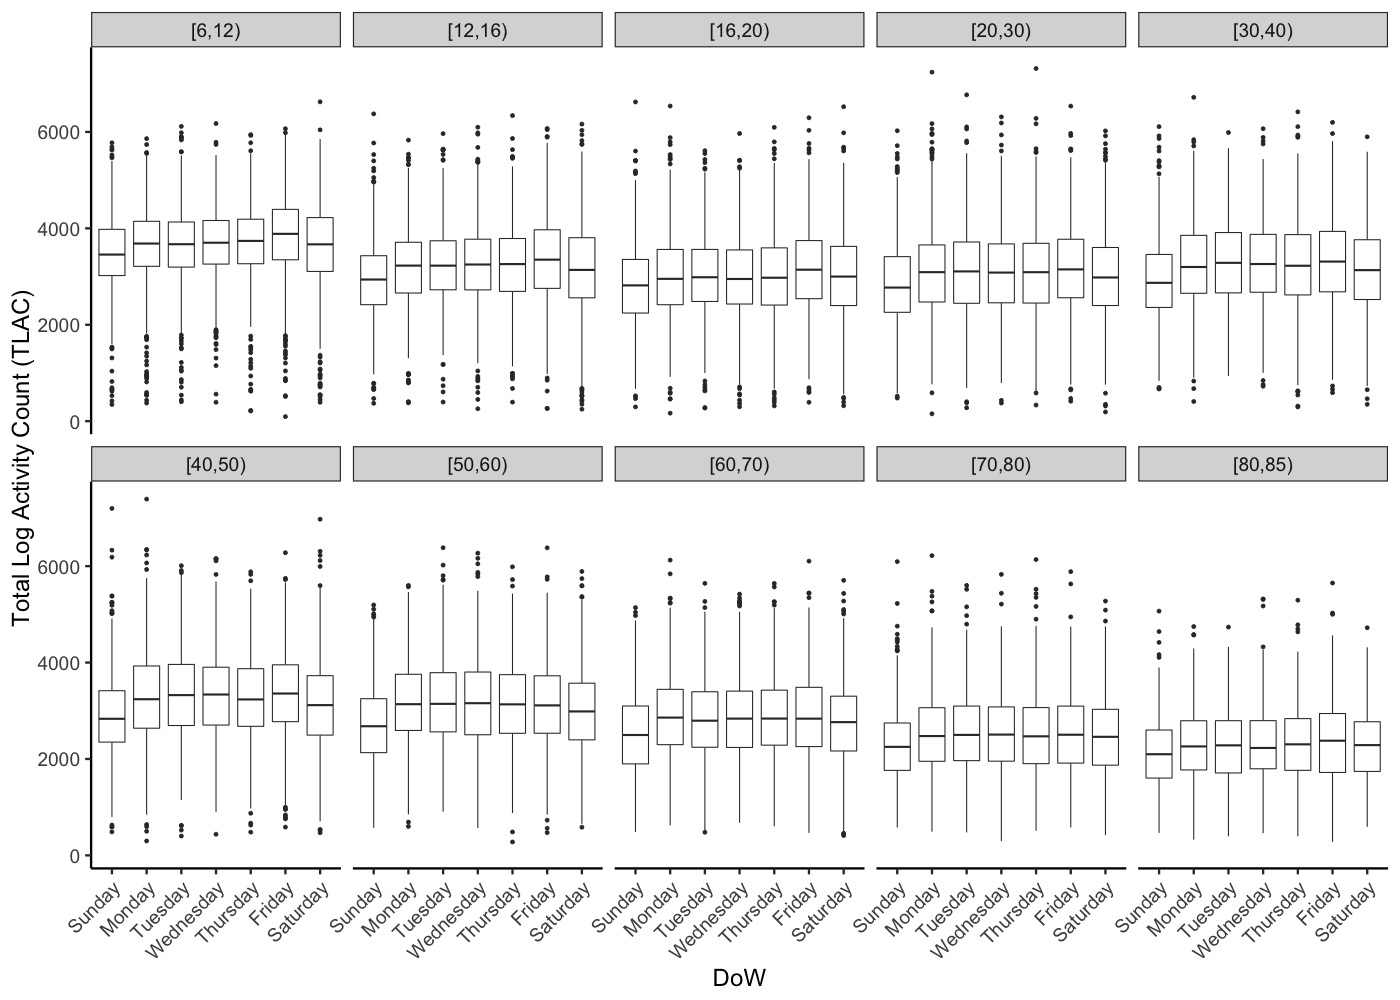
\includegraphics[width=\textwidth]{TLAC_by_age_category}
\end{frame}





\subsection{Feature Extraction}




\begin{frame}
\frametitle{NHANES accelerometry: Features}
\begin{itemize}
\item Current standard: calculate single summaries of the data
    \begin{itemize}
    \item Volume of activity\footnotemark
        \begin{itemize}
        \item Time spent in sedentary/light/moderate/vigorous behaviours. Require population-specific studies to determine thresholds.
        \item Average daily total activity count (TAC). A proxy for total volume of moderate/vigorous activity
        \item Average daily total log activity count (TLAC). A proxy for total volume of low/light activity
        \end{itemize}
    \item Patterns of activity
        \begin{itemize}
        \item Fragmentation measures\footnotemark
        \item Timing of physical activity (activity profiles)
        \end{itemize}
    \end{itemize}
\item Here, we focuse on analyzing patterns of activity using subject-specific average activity profiles and scalar summaries of total volume of activity. 
\end{itemize}


\footnotetext{Varma VR, Dey D, Leroux A, et al. Total volume of physical activity: TAC, TLAC or TAC($\lambda$). Prev Med. 2017;106:233-235.}
\footnotetext{Di, J., Leroux, A., Urbanek, J., et al. Patterns of sedentary and active time accumulation are associated with mortality in US adults: The NHANES study. bioRxiv: 182337.}
\end{frame}




\begin{frame}
\frametitle{Physical Activity and aging}
\begin{itemize}
\item Scientific question: How do patterns of low/light activity change with age? Do these patterns differ between weekends and weekdays? \pause
\item One simple (exploratory) way to look at average patterns of low/light activity as a function of age is to take every individual's average (log) activity profile, for weekends and weekdays separately 
\item Not all participants will contribute to both weekend and weekday estimates! Different number of profiles (days of data) for participants.
\item For simplicity of notation, consider subjects' average profile across all days. 
Let $X_{ij}(t)$ denote the activity count for subject $i = 1,\ldots,N$ on day $j = 1,\ldots,J_i$. 
Then subject $i$'s average profile is: 
    \begin{align*}
    \tilde{X}_i(t) = \frac{1}{J_i}\sum_{j=1}^{J_i} \log[1+X_{ij}(t)], \hspace{0.25cm} t = 1,\ldots,1440
    \end{align*}

\end{itemize}
\end{frame}

\begin{frame}
\frametitle{Physical Activity and aging}
\centering
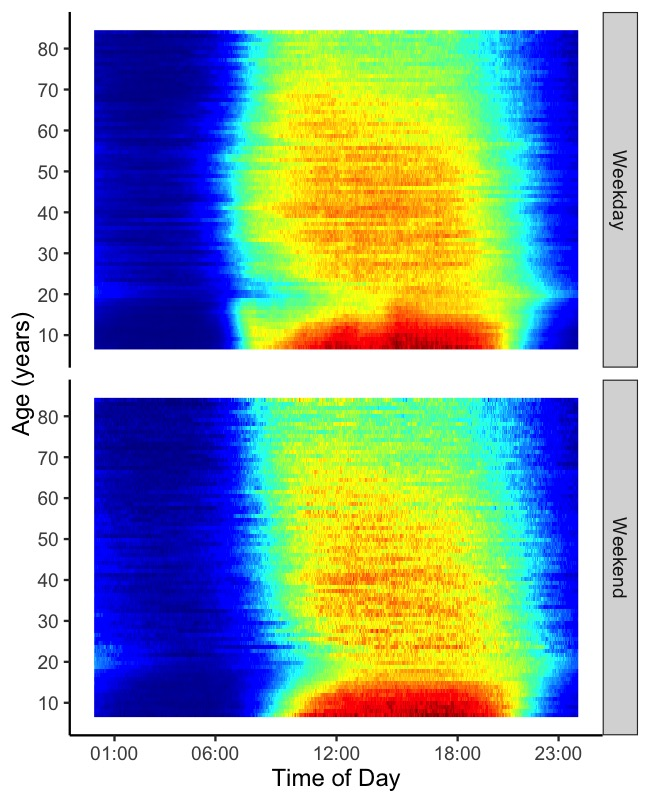
\includegraphics[height=\textheight]{PA_profiles_by_age}
\end{frame}


















\section{Practical Applications}



\begin{frame}
\frametitle{Case study: Prediction of 5-year Mortality}
\begin{itemize}
\item See prediction vignette \url{https://www.github.com/andrew-leroux/CSS_NHANES/vignettes/}
\item Walk through the Rmd file (note: the forward selection code takes a while to run, consider reviewing this section later)
\end{itemize}
\end{frame}



\begin{frame}
\frametitle{Lab Exercises}
\begin{itemize}

\item Walk through Section 1 of "CSS\_NHANES.R", understand data processing, merging, accounting for wear/non-wear, applying exclusion criteria, 
creating simple plots.
\item Work through Section 2 of the "CSS\_NHANES.R" script. Questions:
    \begin{enumerate}
    \item Does average total volume of PA differ between 20-39 year olds in different income-to-needs ratio categories? 
        \begin{itemize}
        \item Exploratory plots (boxplots? histograms?)
        \item Regression analyses 
        \end{itemize}
    \item Does average weekday activity differ between working age (30-54?) among race/ethnicity categories? Can this difference be explained by 
    employment status? Is there a time of day difference?
        \begin{itemize}
        \item One-way and two-way ANOVA for scalar measure of volume of PA?
        \item Bootstrap profiles to estimate differences between certain categories of interest?
        \end{itemize}
    \end{enumerate}
\end{itemize}
\end{frame}






\end{document}
